
\documentclass[a4paper,11pt]{article}

\usepackage[utf8x]{inputenc}
\SetUnicodeOption{mathletters}
\SetUnicodeOption{autogenerated}

\usepackage[italian]{babel}
\usepackage{booktabs}
\usepackage{mathpazo}
\usepackage{graphicx}
\usepackage[left=2cm, right=2cm, bottom=3cm]{geometry}
\frenchspacing

\begin{document}
\noindent {\Large Selezioni nazionali 2010}
\vspace{0.5cm}

\noindent {\Huge Esercizio 3: Pesca bizzarra (\texttt{pesca})}


\vspace{0.5cm}
\noindent {\Large Difficoltà D = 2 (tempo limite 2 sec).}

\section*{Descrizione del problema}
  
Pinco Panco e Panco Pinco hanno deciso di andare a pesca di
ostrichette, ciascuno con la propria barca.
Poiché sanno solo andare in direzione Nord o in direzione Est,
Pinco Panco e Panco Pinco decidono di dividere concettualmente la zona
di pesca in quadrati adiacenti, con i lati nelle direzioni Nord-Sud e
Est-Ovest, ossia disposti come in un foglio a quadretti, e numerati
secondo le coordinate cartesiane intere. Pertanto, ogni quadrato della
griglia è univocamente identificato da una coppia di interi
($I$,$J$), ossia è collocato all'incrocio
della colonna $I$ e della riga $J$ nella suddetta
divisione (dove 1 ≤ $I < 2^{31}$ e 1 ≤
$J < 2^{31}$).

Ciascuna barca si muove soltanto in due direzioni, attraverso uno dei
seguenti \textbf{comandi} numerici, che vengono inviati da una base a
terra:

\begin{itemize}
  
    \item $+D$ (=\textbf{Nord}) per spostarsi dal quadrato
attualmente occupato ($I$,$J$) al quadrato
($I$, $J+D$) attraversando \textbf{tutti} i
$D$-1 quadrati intermedi sulla colonna $I$, dove
$D$ è un intero positivo;
    \item $-D$ (=\textbf{Est}) per spostarsi dal quadrato
attualmente occupato ($I$,$J$) al quadrato
($I+D$, $J$) attraversando \textbf{tutti} i
$D$-1 quadrati intermedi sulla riga $J$, dove
$D$ è un intero positivo;
\end{itemize}

Una sequenza di comandi è quindi una sequenza di interi diversi
da zero che termina con zero.


\begin{figure}[h!]
  \centering
  \caption{}
  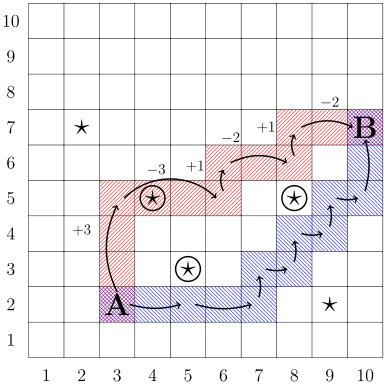
\includegraphics{mare.png}
\end{figure}


Pinco Panco e Panco Pinco utilizzano lo stesso quadrato
A=($I_{0}$,$J_{0}$) di partenza: i
loro sistemi di navigazione sono sincronizzati e ogni barca riceve
dalla base a terra la propria sequenza di comandi con la garanzia che
i quadrati attraversati da entrambe le barche sono solo quello di
partenza A e quello di arrivo B.  Soltanto alcuni dei quadrati sono
pescosi e la base a terra è a conoscenza della loro posizione.

Entrambe le barche iniziano quindi il percorso dal quadrato di
partenza A=($I_{0}$,$J_{0}$) e
ciascuna viene pilotata con la corrispondente sequenza di comandi.
Durante il percorso, ciascuna barca prende un'estremità di
un'enorme rete da pesca (ebbene sì, Pinco Panco e Panco Pinco
usano la rete per pescare le ostrichette!). Le due estremità
dovranno essere ricongiunte nel quadrato di arrivo B: in questo modo,
verranno catturate tutte le ostrichette che si troveranno nella
zona racchiusa dall'enorme rete.

Per esempio, siano $I_{0}$=3 e
$J_{0}$=2. Nella figura, i
$P$=5 quadrati con un asterisco sono pescosi e i
quadrati colorati indicano quelli percorsi delle due barche, con le
sequenze di comandi \texttt{+3 -3 +1 -2 +1 -2 0} e \texttt{-2 -2 +1
-1 +1 -1 +1 -1 +2 0} (notare che possono esserci più
numeri consecutivi dello stesso segno).  Risultano $Q$=3
quadrati pescosi nella zona delimitata dalla rete (quelli identificati
da (4,5), (5,3) e (8,5)).

Aiuta Pinco Panco e Panco Pinco a calcolare il numero $Q$ di
quadrati pescosi che saranno inglobati dalla rete in questo
modo. In tale conteggio, vanno considerati anche i quadrati
attraversati dalle due barche.


\section*{Dati di input}
  Il file \texttt{input.txt} è composto da $P$+4
  righe, dove $P$ è il numero totale di quadrati
  pescosi.

La prima riga contiene un intero $P$ per indicare che la zona
di pesca contiene $P$ quadrati pescosi.

La seconda riga contiene due interi $I_{0}$ e
$J_{0}$ separati da uno spazio, per indicare che il
quadrato di partenza è ($I_{0}$,
$J_{0}$).

Le successive $P$ righe contengono le coordinate dei
$P$ quadrati pescosi. Ogni riga è composta da due
interi $I$ e $J$ separati da uno spazio (dove 1 ≤
$I < 2^{31}$ e 1 ≤ $J <
2^{31}$), per indicare che quel quadrato pescoso ha
coordinate ($I$, $J$).

La penultima riga contiene una sequenza di interi diversi da 0 e
terminata da uno 0, separati da uno spazio: rappresenta la prima
sequenza di comandi (dove 0 è semplicemente utilizzato per
indicare la fine della sequenza di interi).

L'ultima riga contiene anch'essa una sequenza di interi diversi da 0,
terminata da zero, separati da uno spazio: rappresenta la seconda
sequenza di comandi.


\section*{Dati di output}
  
Il file \texttt{output.txt} è composto da una sola riga
contenente il numero $Q$ di quadrati pescosi che sono
inglobati dalla rete.

  \section*{Assunzioni}
  \begin{itemize}
  
    \item $1 ≤ P ≤ 1 000 000$
    \item $1 ≤ I_{0}$ $< 2^{31}$ 
    \item $1 ≤ J_{0}$ $< 2^{31}$ 
    \item Una sequenza di comandi contiene $M$ interi diversi da 0,
per un qualche valore $2 ≤ M ≤ 1 000 000$.
  \end{itemize}

\section*{Esempi di input/output}

  
    \noindent
    \begin{tabular}{p{11cm}|p{5cm}}
    \toprule
    \textbf{File \texttt{input.txt}}
    & \textbf{File \texttt{output.txt}}
    \\
    \midrule
    \scriptsize
    \begin{verbatim}
5
3 2
2 7
4 5
5 3
8 5
9 2
+3 -3 +1 -2 +1 -2 0
-2 -2 +1 -1 +1 -1 +1 -1 +2 0
\end{verbatim}
    &
    \scriptsize
    \begin{verbatim}
3
\end{verbatim}
    \\
    \bottomrule
    \end{tabular}
  
\section*{Nota/e}
\begin{itemize}
  
    \item  
Nessuna.

\end{itemize}



\end{document}
